\subsubsection{Versuchseinführung} % (fold)
\label{ssub:Versuchseinführung}
\begin{frame}
    \frametitle{Versuchseinführung}
    \framesubtitle{}
    \begin{block}{Ziel:}
        Aufnahme eines Elektrokardiogramms am Oszillokops mithilfe von
        Operationsverstärkern
    \end{block}
\end{frame}
\begin{frame}
    \frametitle{Versuchseinführung}
    \framesubtitle{}
    \begin{block}{Definition: EKG}
        Das Elektrokardiogramm (EKG) ist die Aufzeichnung der Summe der elektrischen
        Aktivitäten aller Herzmuskelfasern. Elektrokardiogramm heißt auf
        Deutsch Herzspannungskurve, gelegentlich wird es auch Herzschrift
        genannt.\\ (Quelle: wikipedia.de)
    \end{block}
    \begin{block}{Deshalb notwendig:}
        \begin{itemize}
            \item Empfindlicher Messverstärker der Potenzialunteschiede von
            $10 \mu V$ herausfilter kann
        \end{itemize}
    \end{block}     
\end{frame}

\begin{frame}
    \frametitle{Probleme bei der Messung}
    \framesubtitle{}
    \begin{columns}[c]
    \column{0.5\textwidth}
    \begin{block}{}
        \begin{itemize}
            \item Potentialunterschiede sehr klein
            \pause
            \begin{itemize}
                \item Differenzverstärker mit hoher
                Gleichtaktunterdrückung
            \end{itemize}
        \end{itemize}
    \end{block}
    \column{0.6\textwidth}
    \begin{figure}[H]
    \begin{center}
            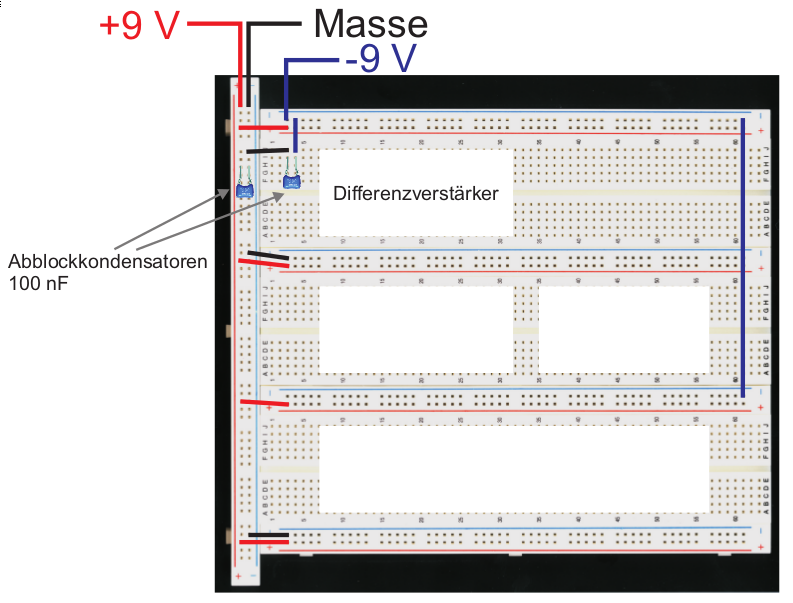
\includegraphics[scale=0.2]{./img/schaltungen/gesamt_0.png}
    \end{center}
    \end{figure}
    \end{columns}
\end{frame}

\begin{frame}
    \frametitle{Probleme bei der Messung}
    \framesubtitle{}
    \begin{columns}[c]
    \column{0.5\textwidth}
    \begin{block}{}
        \begin{itemize}
            \item Potentialunterschiede sehr klein
            \begin{itemize}
                \item Differenzverstärker mit hoher
                Gleichtaktunterdrückung
            \end{itemize}
            \item Signal sehr schwach
            \pause
            \begin{itemize}
                \item Verstärker mit hohem Gesamtverstärkungsfaktor $G=10000$
            \end{itemize}
        \end{itemize}
    \end{block}
    \column{0.6\textwidth}
    \begin{figure}[H]
    \begin{center}
            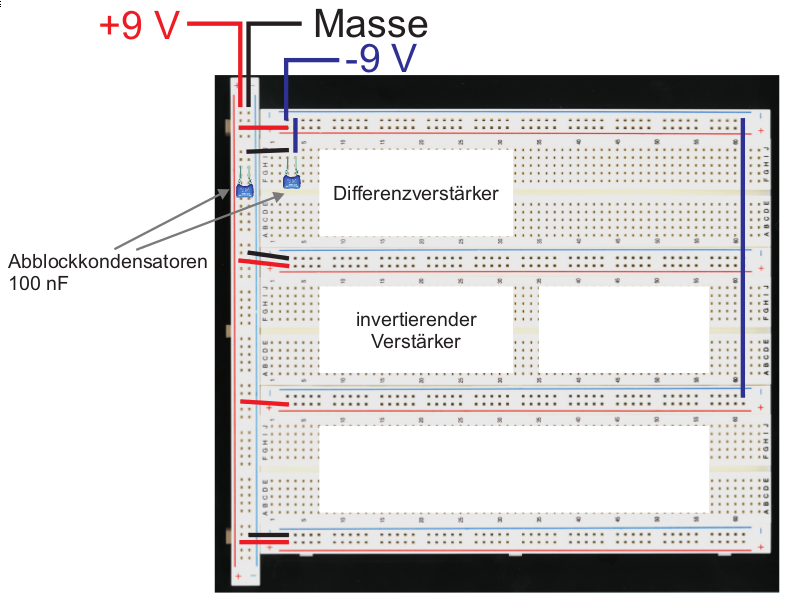
\includegraphics[scale=0.2]{./img/schaltungen/gesamt_1.png}
    \end{center}
    \end{figure}
    \end{columns}
\end{frame}

\begin{frame}
    \frametitle{Probleme bei der Messung}
    \framesubtitle{}
    \begin{columns}[c]
    \column{0.5\textwidth}
    \begin{block}{}
        \begin{itemize}
            \item Potentialunterschiede sehr klein
            \begin{itemize}
                \item Differenzverstärker mit hoher
                Gleichtaktunterdrückung
            \end{itemize}
            \item Signal sehr schwach
            \begin{itemize}
                \item Verstärker mit hohem Gesamtverstärkungsfaktor $G=10000$
            \end{itemize}
            \item DC-Störung
            \pause
            \begin{itemize}
                \item DC-Unterdrückung (Hochpass)
            \end{itemize}
        \end{itemize}
    \end{block}
    \column{0.6\textwidth}
    \begin{figure}[H]
    \begin{center}
            \includegraphics[scale=0.2]{./img/schaltungen/gesamt_2.png}
    \end{center}
    \end{figure}
    \end{columns}
\end{frame}

\begin{frame}
    \frametitle{Probleme bei der Messung}
    \framesubtitle{}
    \begin{columns}[c]
    \column{0.5\textwidth}
    \begin{block}{}
        \begin{itemize}
            \item Potentialunterschiede sehr klein
            \begin{itemize}
                \item Differenzverstärker mit hoher
                Gleichtaktunterdrückung
            \end{itemize}
            \item Signal sehr schwach
                \begin{itemize}
                    \item Verstärker mit hohem Gesamtverstärkungsfaktor $G=10000$
                \end{itemize}
            \item DC-Störung
                \begin{itemize}
                    \item DC-Unterdrückung (Hochpass)
                \end{itemize}
            \item $50Hz$-AC-Störung
            \pause
                \begin{itemize}
                    \item Tiefpass hoher Ordnung
                \end{itemize}
        \end{itemize}
    \end{block}
    \column{0.6\textwidth}
    \begin{figure}[H]
    \begin{center}
            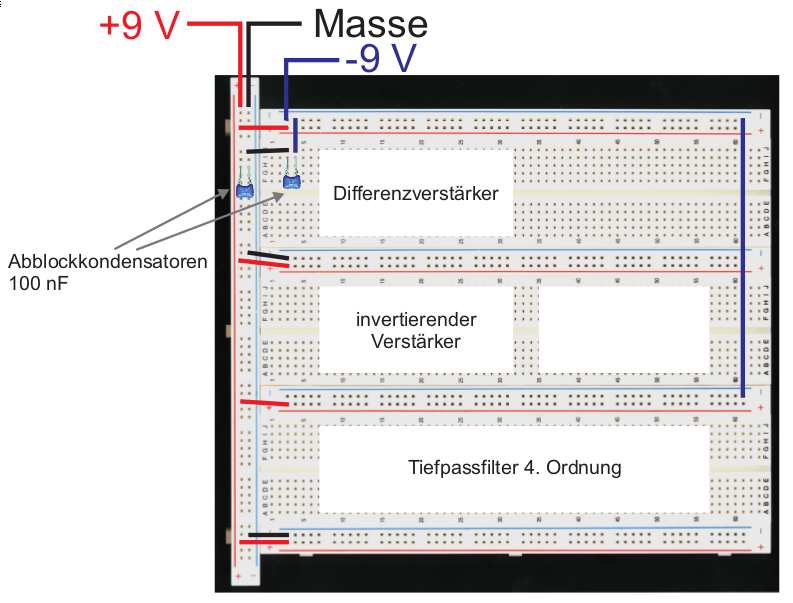
\includegraphics[scale=0.2]{./img/schaltungen/gesamt_3.png}
    \end{center}
    \end{figure}
    \end{columns}
\end{frame}

\begin{frame}
    \frametitle{Probleme bei der Messung}
    \framesubtitle{}
    \begin{columns}[c]
    \column{0.5\textwidth}
    \begin{block}{}
        \begin{itemize}
            \item Potentialunterschiede sehr klein
            \begin{itemize}
                \item Differenzverstärker mit hoher
                Gleichtaktunterdrückung
            \end{itemize}
            \item Signal sehr schwach
                \begin{itemize}
                    \item Verstärker mit hohem Gesamtverstärkungsfaktor $G=10000$
                \end{itemize}
            \item DC-Störung
                \begin{itemize}
                    \item DC-Unterdrückung (Hochpass)
                \end{itemize}
            \item $50Hz$-AC-Störung
                \begin{itemize}
                    \item Tiefpass hoher Ordnung
                \end{itemize}
            \item Visualisierung mit LED
            \pause
                \begin{itemize}
                    \item Komparator
                \end{itemize}        
        \end{itemize}
    \end{block}
    \column{0.6\textwidth}
    \begin{figure}[H]
    \begin{center}
            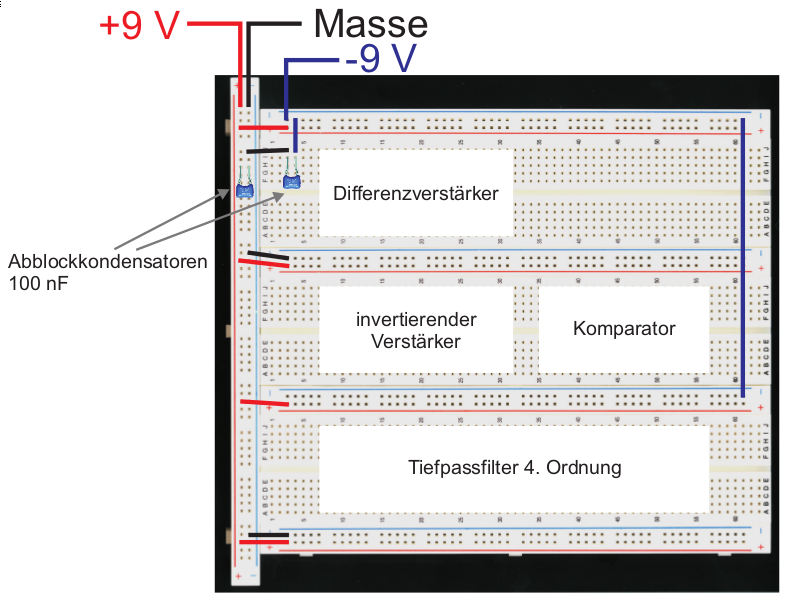
\includegraphics[scale=0.2]{./img/schaltungen/gesamt_4.png}
    \end{center}
    \end{figure}
    \end{columns}
\end{frame}

\begin{frame}
    \frametitle{Gesamtschaltbild}
    \framesubtitle{}
    \begin{figure}[H]
    \begin{center}
            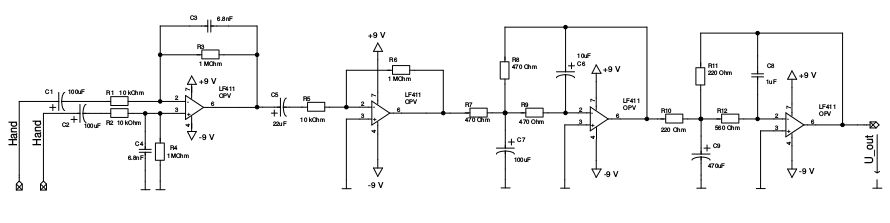
\includegraphics[scale=0.1]{./img/schaltungen/alles_zusammen.png}
    \end{center}
    \end{figure}
\end{frame}
